\chapter{\label{chap:chap4} Metodologia cronograma de desenvolvimento}
% Sérgio: Este capítulo poderia se chamar "Ambiente de simulação e estudos de caso"

% Seção: "Ambiente de simulação" - descrever como tu montou tuas simulações, e como foi organizado o ambiente, etc..

% Seção: "Cenários de teste"

% Seção: "Estudos de caso" (pelo menos 2) - pensar em alguma aplicação, onde por exemplo tens um conjunto amplo de recursos (por exemplo, diversos sensores e atuadores, luminárias, cameras, etc, tipo o prédio 32 da PUC). Pensa que os usuários de tal ambiente (alunos, professores, etc) são potenciais fornecedores de recursos (o alunos é identificado por seu smartphone na rede local e está inscrito em diversas disciplinas). Informações sobre presença (ou ausência) poderiam ser registradas, o aluno poderia ser informado sobre a sala/lab que deveria se dirigir juntamente com o tópico da aula... Sei lá! Tem que pensar em uma forma se simular, de maneira simplificada, um cenário como esse.

Para construção do projeto utilizaremos Python, em sua versão 3.x, como linguagem de programação.
Mais precisamente, utilizaremos a interface de baixo nível de rede da biblioteca padrão da linguagem \cite{socketPython}.
Algumas ferramentas para auxiliar o desenvolvimento serão utilizadas, como Visual Studio Code para edição de código e GitHub para o versionamento.

\begin{figure}[htb!]
    \centering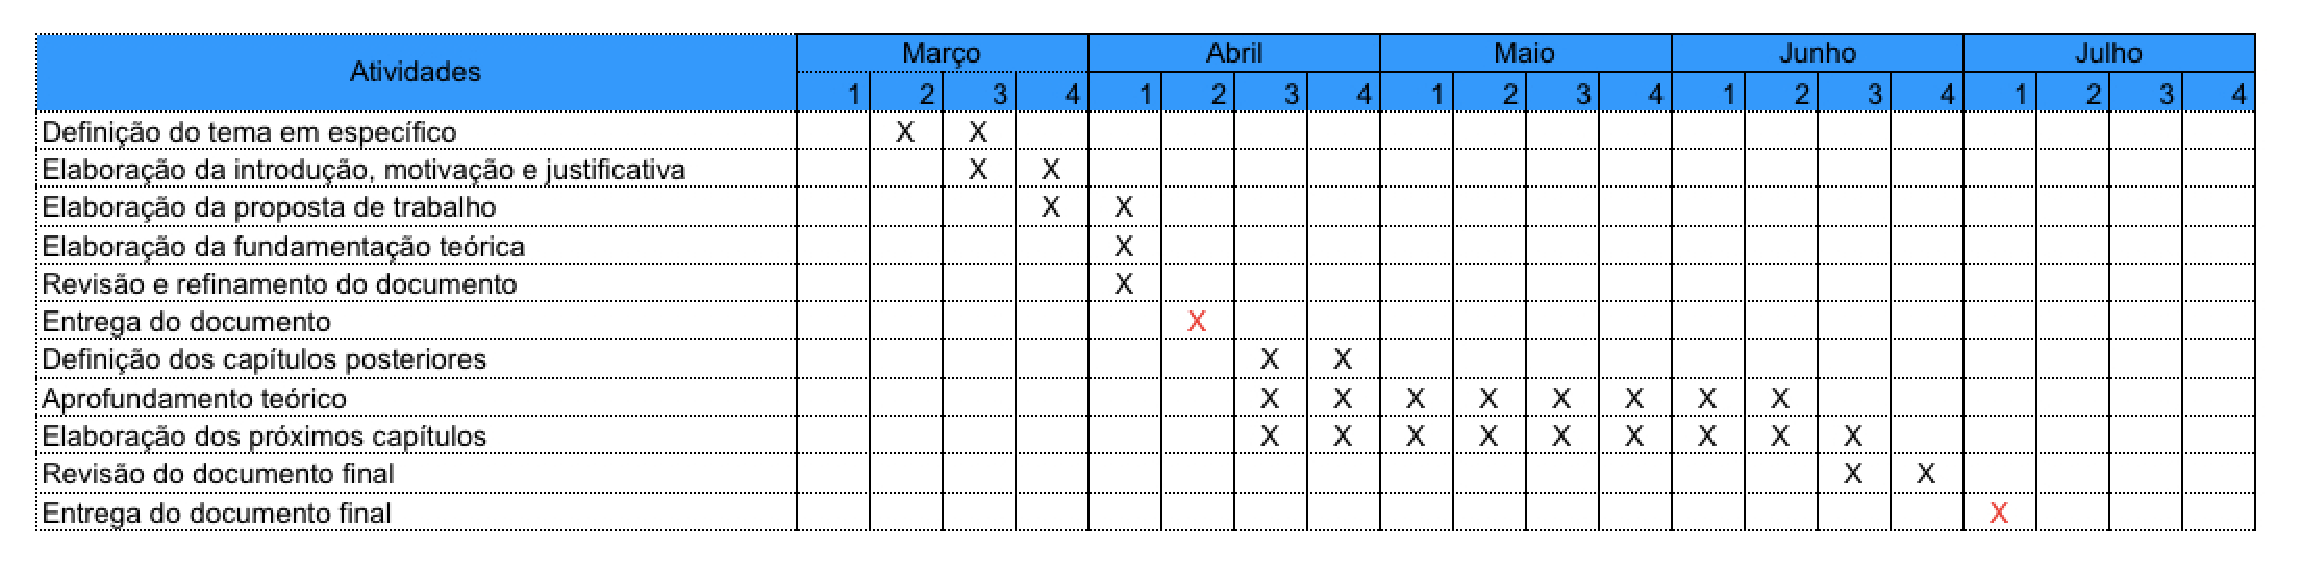
\includegraphics[width=1\textwidth]{fig3.pdf}
    \caption%[This figure has a shorter caption now]%
    {\label{fig:fig3} Cronograma de atividades.}
\end{figure}



